\documentclass[uplatex,dvipdfmx]{jsarticle}

\input{"preamble.tex"}

\title{ヒルベルトの公式に関するメモ}
\author{ガオゾウ}

\begin{document}
\maketitle
\section{概要}
ヒルベルトの公式
\begin{equation}
	\lim_{\eta \to +0}\frac{1}{\omega \pm i\eta} = \pv{\frac{1}{\omega}} \mp i\pi \delta(\omega) \label{eq:formula}
\end{equation}
に関するメモ。ここで$\pv$はコーシーの主値積分を表す。なんかそんな感じの複素積分の公式あったなあと思って何となく使っていたけどいざ示そうと思ったら数弱過ぎてできなかった。悲しい。

この辺の話を数学的にきちんとするとすごくしんどそうなイメージがあるので、全然真面目に証明していません。したがって厳密な証明を期待している方が以下を読むのは推奨いたしません。ご了承下さい。

\section{証明}
式\eqref{eq:formula}はいわゆる超関数の意味での等式であるので、ここでの等号は、各辺を任意の関数\footnote{たぶん本当は積分がちゃんとうまくいくような関数じゃなきゃいけないと思う。数学難しくてよくわからないです。}と積をとって積分\footnote{たぶん実数全体での積分でいい?それとも任意の区間なんだろうか?教えて強い人}した時の結果が必ず一致するという意味であることに注意が必要。この下で式\eqref{eq:formula}を示す。

次の主値積分を考える。
\begin{equation}
	\int_{-\infty}^{\infty} \dd{\omega} \pv{ \frac{\phi(\omega)}{\omega}}
\end{equation}
ここで$\phi(\omega)$はテスト関数で、複素平面全体で正則であり、また$|z|\to \infty$の時$\phi(z)$は十分速く$0$に収束するものとする。このとき、図\ref{fig:contour}のように積分経路$C_1, C_2(赤色円の上半分), C_3(赤色円の下半分)$をとることにすると、
\begin{figure}
	\centering
	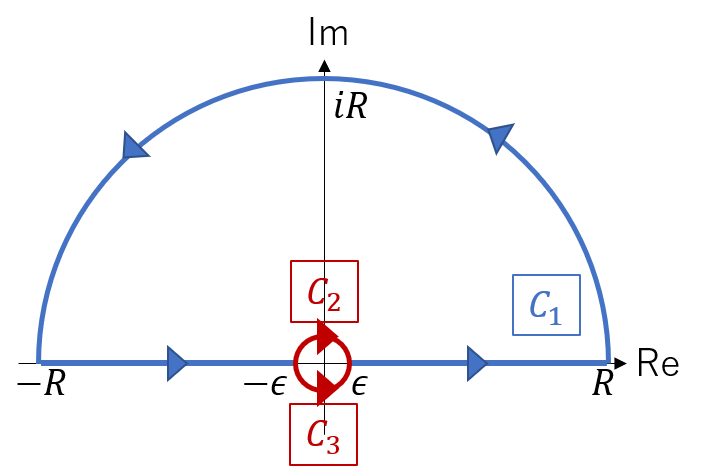
\includegraphics{contour.png}
	\caption{積分経路}
	\label{fig:contour}
\end{figure}

\begin{align}
	\int_{-\infty}^{\infty} \dd{\omega} \pv{\frac{\phi(\omega)}{\omega}} &= \lim_{R\to\infty}\int_{C_1} \dd{z} \frac{\phi(z)}{z} + \lim_{\epsilon\to +0}\qty[\int_{C_i} \dd{z} \frac{\phi(z)}{z}] \pm i\pi \Res_{z=0}(\frac{\phi(z)}{z}) \\
	&= \lim_{R\to\infty, \epsilon\to +0}\int_{C_1+C_i} \dd{z} \qty( \frac{\phi(z)}{z} + \frac{\phi(z)}{z} \pm i\pi \delta(z)\phi(z) ) \\
	&= \lim_{\eta \to +0}\int_{-\infty}^{\infty} \dd{\omega} \qty(\frac{\phi(\omega)}{\omega\pm i\eta}\pm i\pi\delta(\omega)\phi(z) ) \\
	&= \lim_{\eta \to +0}\int_{-\infty}^{\infty} \dd{\omega} \phi(\omega)\qty(\frac{1}{\omega\pm i\eta}\pm i\pi\delta(\omega) )
\end{align}
ここで$\pm$は上が$i=2$のとき、下が$i=3$のときである。
以上から、超関数の意味において、
\begin{align}
	\pv{\frac{\phi(\omega)}{\omega}} &= \frac{1}{\omega \pm i\eta} \pm i\pi\delta(\omega) \\
	\qq{すなわち} \frac{1}{\omega \pm i\eta} &= \pv{\frac{\phi(\omega)}{\omega}} \mp i\pi\delta(\omega)
\end{align}
が示された。
% \begin{align}
% 	\int_{-\infty}^{\infty} \dd{\omega} \pv{\frac{\phi(\omega)}{\omega}} &= \lim_{R\to\infty}\int_{C_1} \dd{z} \frac{\phi(z)}{z} + \frac{1}{2}\lim_{\epsilon\to +0}\qty[\int_{C_2} \dd{z} \frac{\phi(z)}{z} + \int_{C_3} \dd{z} \frac{\phi(z)}{z} ] \\
% 	&= \frac{1}{2}\lim_{R\to\infty, \epsilon\to+0}\qty[\int_{C_1+C_2}\dd{z}\frac{\phi(z)}{z} + \int_{C_1+C_3}\dd{z}\frac{\phi(z)}{z}] \\
% 	&= \frac{1}{2} \lim_{\eta\to 0}	\qty[\int_{-\infty}^{\infty} \dd{\omega} \qty( \frac{\phi(\omega)}{\omega+i\eta} + \frac{\phi(\omega)}{\omega - i\eta})]
% \end{align}



\end{document}